\documentclass[11pt,a4paper]{article}

% ---------- Paquetes ----------
\usepackage{fontspec}
\usepackage[spanish,es-noindentfirst,es-noshorthands]{babel}
\usepackage{geometry}
\geometry{margin=2.3cm}
\usepackage{xcolor}
\usepackage{graphicx}
\usepackage{amsmath}
\usepackage{amssymb}
\usepackage{booktabs}
\usepackage{array}
\usepackage{enumitem}
\usepackage{fancyhdr}
\usepackage{titlesec}
\usepackage[framemethod=default]{mdframed}
\usepackage{listings}
\usepackage{tikz}
\usetikzlibrary{arrows.meta,positioning}
\usepackage{hyperref}
\usepackage{longtable}

% ---------- Colores ----------
\definecolor{azulprof}{HTML}{1F3B73}
\definecolor{azulclaro}{HTML}{E8EEF7}
\definecolor{naranja}{HTML}{C0561E}
\definecolor{verdebox}{HTML}{1E6B3A}
\definecolor{grisclaro}{HTML}{F4F4F4}
\definecolor{codebg}{HTML}{F7F7F2}

\hypersetup{
  colorlinks=true,
  linkcolor=azulprof,
  urlcolor=naranja,
  citecolor=azulprof
}

% ---------- Encabezados ----------
\pagestyle{fancy}
\fancyhf{}
\fancyhead[L]{\small\textcolor{azulprof}{Clasificador de Géneros Musicales}}
\fancyhead[R]{\small\textcolor{azulprof}{Guía de estudio}}
\fancyfoot[C]{\thepage}
\renewcommand{\headrulewidth}{0.4pt}

% ---------- Títulos de sección ----------
\titleformat{\section}
  {\Large\bfseries\color{azulprof}}
  {\thesection.}{0.5em}{}
\titleformat{\subsection}
  {\large\bfseries\color{naranja}}
  {\thesubsection}{0.5em}{}
\titleformat{\subsubsection}
  {\normalsize\bfseries\color{azulprof}}
  {\thesubsubsection}{0.5em}{}

% ---------- Cajas (mdframed) ----------
\mdfdefinestyle{ideastyle}{
  linecolor=azulprof, linewidth=0.8pt,
  backgroundcolor=azulclaro,
  frametitlebackgroundcolor=azulprof,
  frametitlefont=\bfseries\color{white},
  innertopmargin=6pt, innerbottommargin=6pt,
  innerleftmargin=8pt, innerrightmargin=8pt,
  roundcorner=3pt, skipabove=8pt, skipbelow=8pt
}
\mdfdefinestyle{defenstyle}{
  linecolor=verdebox, linewidth=0.8pt,
  backgroundcolor=grisclaro,
  frametitlebackgroundcolor=verdebox,
  frametitlefont=\bfseries\color{white},
  innertopmargin=6pt, innerbottommargin=6pt,
  innerleftmargin=8pt, innerrightmargin=8pt,
  roundcorner=3pt, skipabove=8pt, skipbelow=8pt
}
\newenvironment{ideabox}[1]{\begin{mdframed}[style=ideastyle,frametitle={#1}]}{\end{mdframed}}
\newenvironment{defenbox}[1]{\begin{mdframed}[style=defenstyle,frametitle={#1}]}{\end{mdframed}}

% ---------- Código ----------
\lstset{
  backgroundcolor=\color{codebg},
  basicstyle=\ttfamily\footnotesize,
  keywordstyle=\color{azulprof}\bfseries,
  commentstyle=\color{verdebox}\itshape,
  stringstyle=\color{naranja},
  numbers=left, numberstyle=\tiny\color{gray},
  frame=single, rulecolor=\color{gray!40},
  breaklines=true, showstringspaces=false,
  language=Python, captionpos=b, xleftmargin=14pt
}

\begin{document}

% ================= PORTADA =================
\begin{titlepage}
\centering
\vspace*{2cm}
{\Huge\bfseries\color{azulprof} Clasificador de Géneros Musicales}\\[0.4cm]
{\Large con Inteligencia Artificial}\\[1.2cm]
\rule{0.7\textwidth}{1.5pt}\\[0.6cm]
{\large\itshape Guía de estudio para la defensa final}\\[0.3cm]
{\large Análisis de audio con \texttt{librosa}, SVM y Redes Neuronales}\\[2cm]

\begin{mdframed}[linecolor=azulprof,backgroundcolor=azulclaro,linewidth=0.8pt,roundcorner=3pt,innermargin=0pt,leftmargin=30pt,rightmargin=30pt,innertopmargin=10pt,innerbottommargin=10pt]
\centering
Este documento explica \textbf{en profundidad} cómo funciona cada etapa del
proyecto: desde la física del sonido y cómo \texttt{librosa} extrae las
características, hasta por qué los modelos asocian el folklore con
\emph{country} o \emph{música clásica}.
\end{mdframed}

\vfill
{\large Inteligencia Artificial --- 2025}\\
{\normalsize Universidad Nacional de Río Cuarto}\\[0.5cm]
{\small Documento generado para estudio grupal}
\end{titlepage}

\tableofcontents
\newpage

% ================= 1. INTRODUCCION =================
\section{Introducción y objetivos}

El proyecto es un \textbf{clasificador automático de géneros musicales}. La idea
central es: tomar un archivo de audio, convertirlo en una lista de números que
describen sus propiedades acústicas (las \emph{features}), y entrenar un modelo
de Machine Learning que aprenda a asociar esos números con un género.

\begin{ideabox}{La pregunta de investigación}
No buscamos solo ``acertar el género''. Lo interesante es \textbf{entender por
qué} el modelo decide lo que decide. En particular: ¿qué pasa cuando le mostramos
folklore argentino, un género que el modelo nunca vio? ¿Por qué lo confunde con
\emph{country} o \emph{clásica}?
\end{ideabox}

\subsection{Los dos experimentos}

\begin{description}[leftmargin=1.2cm,style=nextline]
  \item[Experimento A --- Folklore \emph{sin} entrenar]
  Entrenamos un SVM solo con el dataset GTZAN (10 géneros internacionales) y
  luego le pedimos que clasifique canciones de folklore argentino. Como el
  modelo no conoce ``folklore'', se ve \emph{obligado} a encajarlo en alguno de
  los 10 géneros que sí conoce. El resultado revela qué géneros ``suenan
  parecido'' al folklore según las features.

  \item[Experimento B --- Folklore \emph{con} entrenamiento]
  Agregamos 70 canciones de folklore como un género nuevo (\#11), reentrenamos
  y evaluamos con \emph{cross-validation} sobre canciones que quedaron fuera del
  entrenamiento. El modelo reconoce el folklore $\sim$66\% de las veces:
  demuestra que las features \textbf{sí} capturan la identidad del género, solo
  faltaban ejemplos.
\end{description}

Adicionalmente se entrena una \textbf{Red Neuronal} (perceptrón multicapa) sobre
las mismas features para comparar con el SVM, y existe un experimento con
\textbf{CNN} sobre espectrogramas (descartado en principio, pero documentado al
final).

\subsection{Pipeline general}

\begin{center}
\begin{tabular}{c c c c c}
\textbf{Audio} & $\rightarrow$ & \textbf{Features} & $\rightarrow$ & \textbf{Modelo} \\
\texttt{.wav / .mp3} & & 45 números (librosa) & & SVM / Red Neuronal \\
\end{tabular}
\end{center}

\begingroup\footnotesize\renewcommand{\_}{\textunderscore\allowbreak}
\begin{longtable}{p{3.6cm} p{3.3cm} p{6cm}}
\toprule
\textbf{Script} & \textbf{Etapa} & \textbf{Qué hace} \\
\midrule
\texttt{features.py} & Módulo común & Funciones compartidas: \texttt{extract\_features} y la carga del folklore con cache \\
\texttt{1\_data\_extraction.py} & Extracción & Recorre GTZAN, extrae 45 features por canción $\rightarrow$ \texttt{my\_features.csv} \\
\texttt{2\_model\_training.py} & Entrenamiento & Entrena SVM (RBF), guarda modelo + scaler + label encoder \\
\texttt{3\_folklore\_analysis.py} & Experimento A & Predice folklore con el SVM sin reentrenar \\
\texttt{4\_folklore\_training\_and\_testing.py} & Experimento B (demo) & Reentrena con folklore incluido y prueba con 1 canción no vista \\
\texttt{5\_folklore\_crossvalidation.py} & Experimento B & Evalúa el folklore con \emph{cross-validation} 5-fold (versión correcta) \\
\texttt{6\_model\_comparison.py} & Comparación justa & SVM vs Red Neuronal sobre el mismo split (11 clases) \\
\bottomrule
\end{longtable}
\endgroup

% ================= ESTADO DEL PROYECTO =================
\section{Estado del proyecto: modelos, datos y archivos}

Antes de entrar en los detalles, este es el ``mapa'' del proyecto: qué se genera,
qué modelos quedan guardados y qué archivos hacen falta para cada cosa.

\subsection{El flujo de datos}

\begin{center}
\begin{tikzpicture}[
  box/.style={rectangle, draw=azulprof, fill=azulclaro, rounded corners,
    align=center, minimum height=0.9cm, text width=2.5cm, font=\scriptsize},
  io/.style={rectangle, draw=naranja, fill=white, rounded corners,
    align=center, minimum height=0.9cm, text width=2.0cm, font=\scriptsize},
  >=Stealth, node distance=0.6cm and 0.9cm
]
\node[io] (gtzan) {Audio GTZAN};
\node[io, below=of gtzan] (folk) {Audio folklore};
\node[box, right=of gtzan] (csv1) {\texttt{my\_features}\\\texttt{.csv}};
\node[box, right=of folk]  (csv2) {\texttt{folklore\_}\\\texttt{features.csv}};
\node[box, right=of csv1, yshift=-0.75cm] (model) {Modelos\\SVM / Red};
\node[box, right=of model] (exp) {Experimentos\\y predicciones};
\draw[->] (gtzan) -- node[above,font=\tiny]{script 1} (csv1);
\draw[->] (folk)  -- node[above,font=\tiny]{features.py} (csv2);
\draw[->] (csv1) -- (model);
\draw[->] (csv2) -- (model);
\draw[->] (model) -- node[above,font=\tiny]{2, 4, 5, 6} (exp);
\end{tikzpicture}
\end{center}

Hay \textbf{dos} fuentes de audio que se extraen \textbf{por separado}, y este es
un punto que suele confundir:
\begin{itemize}[leftmargin=0.7cm]
  \item \textbf{GTZAN}: lo extrae \texttt{1\_data\_extraction.py} una sola vez
  $\rightarrow$ \texttt{my\_features.csv} (999 canciones, 45 features c/u).
  \item \textbf{Folklore}: el script 1 \textbf{no} lo procesa. Lo cargan los
  scripts de folklore (3, 4, 5 y 6) a través de \texttt{features.py}, que extrae
  desde la carpeta de folklore \textbf{una sola vez} y guarda
  \texttt{folklore\_\allowbreak features.csv} (70 canciones). En las corridas siguientes se
  lee del cache.
\end{itemize}

Una vez que las features están en los CSVs, el entrenamiento y los experimentos
(scripts 2, 4, 5 y 6) ya \textbf{no} tocan el audio.

\begin{ideabox}{Extracción centralizada (refactor)}
La función \texttt{extract\_features} estaba \textbf{copiada} en varios scripts, y
los scripts 3 y 4 re-extraían el folklore en cada corrida. Se centralizó todo en
el módulo \texttt{features.py}: una única \texttt{extract\_\allowbreak features} y una función
\texttt{load\_\allowbreak folklore\_\allowbreak features} con cache. Ahora todos los scripts importan de
ahí, no hay código duplicado y el audio del folklore se procesa una sola vez.
\end{ideabox}

\subsection{Los modelos guardados (y por qué son 3 archivos cada uno)}

Algo que confunde al principio: \textbf{cada ``modelo'' son en realidad 3
archivos} que viajan juntos. No alcanza con el clasificador solo; para predecir
el género de una canción se necesitan los tres:

\begin{center}
\begin{tabular}{p{3.2cm} p{3cm} p{7.5cm}}
\toprule
\textbf{Archivo} & \textbf{Qué es} & \textbf{Para qué sirve} \\
\midrule
\texttt{svm\_*.pkl} & Clasificador SVM & Hace la predicción del género \\
\texttt{scaler\_*.pkl} & \texttt{StandardScaler} & Normaliza las features de una canción nueva \emph{igual} que en el entrenamiento. Sin esto, los números entran en otra escala y el modelo falla \\
\texttt{label\_\allowbreak encoder\_*.pkl} & \texttt{LabelEncoder} & Traduce entre el número interno del modelo y el nombre del género ($0 \leftrightarrow$ blues, $4 \leftrightarrow$ folklore, \ldots) \\
\bottomrule
\end{tabular}
\end{center}

En la carpeta \texttt{models/} hay \textbf{dos modelos}, ambos SVM:

\begin{center}
\begin{tabular}{p{4.5cm} c p{7cm}}
\toprule
\textbf{Modelo (trío)} & \textbf{Clases} & \textbf{Qué hace} \\
\midrule
\texttt{svm\_model} (+ scaler, encoder) & 10 (GTZAN) & Clasificador base. Es el del \textbf{Experimento A}: predice folklore con géneros que ya conoce ($\rightarrow$ \emph{country}) \\
\texttt{svm\_with\_folklore} (+ \ldots) & 11 (GTZAN + folk) & El que sí conoce ``folklore'' como clase. Modelo final del \textbf{Experimento B} \\
\bottomrule
\end{tabular}
\end{center}

\begin{defenbox}{La red neuronal no se guarda en disco}
Los únicos modelos persistidos son los \textbf{dos SVM}. La \textbf{red neuronal}
se entrena en memoria dentro del script de comparación (se usa y se descarta en
cada corrida). Esto es a propósito: el foco del proyecto es el \emph{análisis},
no servir predicciones en producción.
\end{defenbox}

\subsection{¿Hace falta el audio una vez que tengo el CSV?}

\textbf{Para reproducir los experimentos y entrenar: no.} Los scripts 2, 4, 5
y 6 \textbf{solo leen los CSVs}, nunca abren un \texttt{.wav}. Con los CSVs
alcanza para reentrenar todo y reproducir cada resultado.

\textbf{El audio sí se necesita en dos casos:}
\begin{enumerate}[leftmargin=0.8cm]
  \item \textbf{Re-extraer features}: si cambiás qué features usás, o
  agregás/quitás canciones, hay que volver a correr la extracción sobre los
  \texttt{.wav}.
  \item \textbf{Clasificar una canción nueva}: el modelo no ``come'' audio, come
  el vector de 45 números. Para una canción que no está en el CSV, primero hay
  que extraerle las features desde su \texttt{.wav}.
\end{enumerate}

En resumen, el audio pasa a ser \textbf{materia prima}: para lo ya hecho no se
necesita; para extender el dataset o probar canciones nuevas, sí.

\subsection{Resumen del estado actual}

\begin{center}
\begin{tabular}{p{6.5cm} c p{5cm}}
\toprule
\textbf{Componente} & \textbf{Estado} & \textbf{Detalle} \\
\midrule
Extracción de features (script 1) & \checkmark & 45 features con librosa \\
SVM base (10 géneros) & \checkmark & $\sim$68\% accuracy \\
SVM con folklore (11 clases) & \checkmark & guardado en \texttt{models/} \\
Experimento A (folklore sin entrenar) & \checkmark & cae en \emph{country} \\
Experimento B + cross-validation & \checkmark & recall 65.7\% $\pm$ 9.5\% \\
Red neuronal + comparación justa & \checkmark & empata con SVM ($\sim$66--68\%) \\
Documentación (este PDF) & \checkmark & guía de estudio completa \\
CNN & descartada & solo queda el script de referencia \\
\bottomrule
\end{tabular}
\end{center}

% ================= 2. SONIDO Y LIBROSA =================
\section{Cómo funciona \texttt{librosa} en profundidad}

Este es uno de los puntos que el profesor remarcó: entender de verdad qué hace
la librería, no usarla como una caja negra.

\subsection{Qué es una señal de audio digital}

El sonido es una onda de presión que varía en el tiempo. Para procesarla en una
computadora se \textbf{muestrea}: se mide la amplitud de la onda muchas veces por
segundo. Ese ritmo de muestreo es el \textbf{sample rate} ($sr$).

\begin{lstlisting}
y, sr = librosa.load(file_path, duration=30, sr=22050)
\end{lstlisting}

\begin{itemize}[leftmargin=0.7cm]
  \item \texttt{y} es un arreglo de NumPy con las amplitudes de la onda. Si
  cargamos 30 segundos a 22050 Hz, \texttt{y} tiene
  $30 \times 22050 = 661{,}500$ números.
  \item \texttt{sr = 22050} significa \textbf{22050 muestras por segundo}.
  \texttt{librosa} usa este valor por defecto (la mitad del estándar de CD,
  44100 Hz). Es suficiente porque por el \emph{teorema de Nyquist} permite
  representar frecuencias hasta $sr/2 = 11025$ Hz, que cubre casi toda la
  energía musical relevante.
  \item \texttt{duration=30} recorta a los primeros 30 segundos (igual que
  GTZAN, donde cada clip dura 30 s).
\end{itemize}

\begin{ideabox}{¿Por qué fijar el sample rate?}
Si distintas canciones se cargaran a distintos \emph{sample rates}, las features
no serían comparables. Fijar \texttt{sr=22050} garantiza que todas las
canciones se analizan en la misma ``resolución temporal''.
\end{ideabox}

\subsection{El paso clave: de la onda al espectro (STFT)}

La onda cruda (dominio del tiempo) dice \emph{cuándo} suena fuerte, pero no
\emph{qué frecuencias} contiene. Para eso se aplica la
\textbf{Transformada de Fourier de Tiempo Corto (STFT)}:

\begin{enumerate}[leftmargin=0.8cm]
  \item Se parte la señal en \textbf{ventanas} cortas que se solapan
  (típicamente de 2048 muestras, avanzando de a 512 --- el \texttt{hop\_length}).
  \item A cada ventana se le aplica la \textbf{Transformada de Fourier}, que la
  descompone en sus frecuencias componentes (¿cuánta energía hay en los graves,
  en los medios, en los agudos?).
  \item El resultado es un \textbf{espectrograma}: una matriz
  \emph{frecuencia $\times$ tiempo} donde cada celda dice cuánta energía hay en
  esa frecuencia en ese instante.
\end{enumerate}

\begin{ideabox}{Idea central}
Casi todas las features de \texttt{librosa} (MFCC, chroma, centroide, rolloff,
bandwidth) se calculan \textbf{a partir del espectrograma}. Entender el
espectrograma es entender el 80\% de la librería.
\end{ideabox}

\subsection{El truco mean/std: de una matriz a un número}

Un espectrograma de 30 segundos tiene cientos de columnas (una por ventana
temporal). Pero el SVM necesita un \textbf{vector de tamaño fijo} por canción.
La solución del proyecto es \textbf{resumir cada feature en el tiempo} usando su
media (\texttt{np.mean}) y a veces su desviación estándar (\texttt{np.std}):

\begin{lstlisting}
mfcc = librosa.feature.mfcc(y=y, sr=sr, n_mfcc=13)  # shape (13, ~1300)
mfcc_mean = np.mean(mfcc, axis=1)   # 13 numeros: promedio temporal
mfcc_std  = np.std(mfcc, axis=1)    # 13 numeros: cuanto varia en el tiempo
\end{lstlisting}

\begin{itemize}[leftmargin=0.7cm]
  \item \texttt{axis=1} promedia \textbf{a lo largo del tiempo}, dejando un valor
  por banda.
  \item La \textbf{media} captura el ``valor típico'' de esa propiedad en la
  canción.
  \item La \textbf{desviación estándar} captura cuánto \emph{varía}: una canción
  con muchos cambios dinámicos tendrá std alto.
\end{itemize}

\begin{defenbox}{Limitación a mencionar en la defensa}
Al promediar en el tiempo \textbf{perdemos la estructura temporal} de la canción
(estrofa, estribillo, silencios). Para el SVM esto es necesario, pero es
justamente lo que una CNN o un modelo recurrente podrían aprovechar.
\end{defenbox}

% ================= 3. LAS FEATURES =================
\section{Las 45 features, una por una}

Cada canción se convierte en un vector de \textbf{45 números}. Esta tabla los
agrupa; luego explicamos las más importantes.

\begin{longtable}{p{3.6cm} c p{7.5cm}}
\toprule
\textbf{Feature} & \textbf{\#} & \textbf{Qué describe} \\
\midrule
MFCC (mean) & 13 & Forma del espectro $\rightarrow$ \textbf{timbre} (valor típico) \\
MFCC (std) & 13 & Variación del timbre a lo largo de la canción \\
Chroma & 12 & Energía en cada una de las 12 notas $\rightarrow$ \textbf{armonía} \\
Spectral Centroid (mean/std) & 2 & ``Brillo'': dónde está el centro de masa del espectro \\
Spectral Rolloff (mean) & 1 & Frecuencia bajo la cual está el 85\% de la energía \\
Spectral Bandwidth (mean) & 1 & ``Ancho'' del espectro alrededor del centroide \\
Zero Crossing Rate (mean) & 1 & Cuántas veces la onda cruza el cero (ruido/percusión) \\
Tempo & 1 & Velocidad estimada en BPM \\
RMS Energy (mean) & 1 & Energía/volumen promedio \\
\midrule
\textbf{Total} & \textbf{45} & \\
\bottomrule
\end{longtable}

\subsection{MFCC --- la feature estrella (análisis en profundidad)}

El profesor pidió investigar al menos una feature a fondo. Los \textbf{MFCC}
(\emph{Mel-Frequency Cepstral Coefficients}) son la mejor candidata: son las más
importantes para el modelo y las más interesantes conceptualmente.

\subsubsection{¿Qué problema resuelven?}

Queremos describir el \textbf{timbre}: eso que hace que una guitarra y un piano
tocando la misma nota suenen distinto. El timbre está en la \emph{forma} de la
envolvente del espectro (qué armónicos resalta el instrumento), no en la nota en
sí.

\subsubsection{Cómo se calculan (paso a paso)}

\begin{enumerate}[leftmargin=0.8cm]
  \item \textbf{Espectrograma} vía STFT (visto antes).
  \item \textbf{Escala Mel}: las frecuencias se reagrupan según la
  \emph{escala Mel}, que imita cómo el oído humano percibe el tono. Distinguimos
  muy bien los graves pero comprimimos los agudos: la escala Mel hace lo mismo.
  \item \textbf{Logaritmo}: se toma el log de la energía, porque percibimos el
  volumen de forma logarítmica (decibeles).
  \item \textbf{DCT} (Transformada Coseno Discreta): comprime todo en unos pocos
  coeficientes que describen la \emph{forma} de la envolvente espectral.
  Conservamos los primeros 13 (\texttt{n\_mfcc=13}).
\end{enumerate}

\begin{ideabox}{Interpretación de los coeficientes}
\begin{itemize}[leftmargin=0.5cm]
  \item El \textbf{MFCC 0} se relaciona con la \textbf{energía global} del frame.
  \item Los \textbf{coeficientes bajos} (1--4) capturan la forma gruesa del
  espectro (¿es un sonido ``oscuro'' o ``brillante''?).
  \item Los \textbf{coeficientes altos} (5--12) capturan detalles finos del
  timbre.
\end{itemize}
Por eso son tan buenos separando \emph{metal} (distorsión, mucha energía en
agudos) de \emph{classical} (timbre suave de cuerdas y maderas).
\end{ideabox}

\subsection{Chroma --- la armonía y las notas}

\texttt{chroma\_stft} colapsa todas las octavas en las \textbf{12 clases de
notas} (Do, Do\#, Re, ..., Si). Cada uno de los 12 valores indica cuánta energía
hay en esa nota a lo largo de la canción. Captura la \textbf{armonía}: qué
acordes y tonalidades predominan. Es clave para géneros con armonía marcada
(jazz, clásica) frente a otros más rítmicos o ruidosos (metal, hiphop).

\subsection{Features espectrales --- el ``color'' del sonido}

\begin{description}[leftmargin=0.5cm,style=nextline]
  \item[Spectral Centroid (brillo)] Es el ``centro de masa'' del espectro. Si
  hay mucha energía en agudos, el centroide es alto y el sonido se percibe
  \emph{brillante} (metal, pop electrónico). Si predominan los graves, es bajo y
  suena \emph{oscuro} (clásica, jazz suave).
  \item[Spectral Rolloff] La frecuencia por debajo de la cual se acumula el 85\%
  de la energía. Distingue sonidos con mucho contenido en agudos de los más
  ``apagados''.
  \item[Spectral Bandwidth] Cuán ``ancho'' es el espectro alrededor del
  centroide. Sonidos ruidosos/distorsionados tienen bandwidth alto; tonos puros,
  bajo.
\end{description}

\subsection{Features temporales --- ritmo y energía}

\begin{description}[leftmargin=0.5cm,style=nextline]
  \item[Zero Crossing Rate (ZCR)] Cuántas veces por segundo la onda cruza el
  cero. Es alto en sonidos ruidosos/percusivos (platillos, distorsión, voz
  fricativa) y bajo en tonos limpios. Útil para detectar percusión.
  \item[Tempo (BPM)] \texttt{librosa.beat.beat\_track} estima la velocidad
  detectando picos periódicos de energía (los ``golpes''). Separa baladas lentas
  de música bailable.
  \item[RMS Energy] La raíz cuadrática media de la amplitud: el ``volumen''
  promedio. Géneros agresivos (metal) tienen RMS alto y constante; la clásica
  tiene mucha variación dinámica.
\end{description}

\subsection{Por qué se normaliza (StandardScaler)}

Las features viven en escalas muy distintas: el tempo ronda 60--180, el ZCR está
entre 0 y 1, el rolloff llega a miles de Hz. Sin normalizar, el SVM le daría
\emph{artificialmente} más importancia a las features con números grandes.

\begin{lstlisting}
scaler = StandardScaler()
X_train_scaled = scaler.fit_transform(X_train)  # media 0, std 1
X_test_scaled  = scaler.transform(X_test)        # MISMA transformacion
\end{lstlisting}

\begin{defenbox}{Detalle importante}
El scaler se ajusta (\texttt{fit}) \textbf{solo con el train} y luego se
\emph{aplica} al test. Si se ajustara con todo, habría ``data leakage'': el
modelo vería información del test durante el entrenamiento. Por eso el scaler se
guarda en \texttt{models/scaler.pkl} y se reutiliza con el folklore.
\end{defenbox}

% ================= 4. SVM =================
\section{Modelo 1: SVM (Support Vector Machine)}

\subsection{Idea intuitiva}

Un SVM busca el \textbf{hiperplano} que mejor separa dos clases, maximizando el
\emph{margen} (la distancia a los puntos más cercanos de cada clase, llamados
\textbf{vectores de soporte}). Cuanto más ancho el margen, mejor generaliza.

\subsection{El kernel RBF: por qué es no lineal}

Nuestras 45 features no se separan con líneas rectas. El \textbf{kernel RBF}
(\emph{Radial Basis Function}) resuelve esto midiendo \textbf{similitud por
cercanía}:
\[
K(x_i, x_j) = \exp\!\left(-\gamma \, \lVert x_i - x_j \rVert^2\right)
\]
Dos canciones con features parecidas (distancia chica) tienen $K \approx 1$; muy
distintas, $K \approx 0$. Esto equivale a proyectar los datos a un espacio de
dimensión altísima donde \emph{sí} se pueden separar con un hiperplano. El
resultado son fronteras \textbf{curvas} en el espacio original.

\begin{lstlisting}
model = SVC(kernel='rbf', random_state=42, probability=True)
model.fit(X_train_scaled, y_train)
\end{lstlisting}

\begin{itemize}[leftmargin=0.7cm]
  \item \texttt{probability=True} permite obtener \texttt{predict\_proba}: la
  ``confianza'' del modelo en cada género. Es lo que usamos para ver qué tan
  seguro está al clasificar folklore.
  \item \texttt{random\_state=42} hace el experimento \textbf{reproducible}.
\end{itemize}

\subsection{Multiclase: 10 géneros con un clasificador binario}

El SVM es binario por naturaleza. Scikit-learn lo extiende con la estrategia
\textbf{one-vs-one}: entrena un SVM por cada par de géneros
($\binom{10}{2}=45$ clasificadores) y vota. El género más votado gana.

\subsection{Resultados del SVM (GTZAN)}

\begin{center}
\begin{tabular}{l c c c}
\toprule
\textbf{Género} & \textbf{Precision} & \textbf{Recall} & \textbf{F1} \\
\midrule
Classical & 0.947 & 0.900 & 0.923 \\
Jazz      & 0.731 & 0.950 & 0.826 \\
Pop       & 0.762 & 0.800 & 0.780 \\
Metal     & 0.875 & 0.700 & 0.778 \\
Country   & 0.667 & 0.700 & 0.683 \\
Blues     & 0.619 & 0.650 & 0.634 \\
Rock      & 0.714 & 0.500 & 0.588 \\
Reggae    & 0.611 & 0.550 & 0.579 \\
Hiphop    & 0.478 & 0.550 & 0.512 \\
Disco     & 0.476 & 0.500 & 0.488 \\
\midrule
\textbf{Accuracy global} & \multicolumn{3}{c}{\textbf{\textasciitilde 68\%}} \\
\bottomrule
\end{tabular}
\end{center}

\begin{ideabox}{Cómo leer estos números}
\textbf{Precision}: de todo lo que predije como ``X'', cuánto era realmente X.
\textbf{Recall}: de todo lo que era realmente X, cuánto detecté.
\textbf{F1}: media armónica de ambos. \texttt{Classical} casi perfecto (timbre
muy distintivo); \texttt{disco}/\texttt{hiphop} se confunden entre sí (beats
electrónicos similares). El 68\% es bueno: el azar daría 10\%.
\end{ideabox}

% ================= 5. EXPERIMENTOS FOLKLORE =================
\section{El corazón del proyecto: por qué el modelo confunde el folklore}

Aquí está la parte que el profesor quiere que entendamos de verdad: \textbf{por
qué} el modelo ``mira'' al folklore de cierta forma.

\subsection{Experimento A: folklore sin entrenar}

El SVM solo conoce 10 géneros. Al darle folklore, \texttt{predict} lo fuerza a
elegir el ``más parecido'' según las features. Resultado típico: la mayoría cae
en \textbf{country}, y algunas canciones con violín o cuerdas en
\textbf{classical}.

\begin{defenbox}{La explicación acústica (clave de la defensa)}
El modelo \textbf{no entiende de cultura}; solo compara números. El folklore
comparte con esos géneros sus \textbf{features superficiales}:
\begin{itemize}[leftmargin=0.5cm]
  \item \textbf{Folklore $\rightarrow$ country}: ambos usan \textbf{guitarra
  acústica}, estructuras armónicas simples (pocos acordes $\rightarrow$ chroma
  parecido) y tempos medios (90--140 BPM). Los MFCC del timbre de guitarra
  acústica caen cerca de los del country.
  \item \textbf{Folklore con violín $\rightarrow$ classical}: el violín produce
  un timbre de cuerda frotada (MFCC) y un centroide espectral parecidos a los de
  la música clásica. El modelo ``ve'' cuerdas y dispara classical.
\end{itemize}
Conclusión: el modelo captura \textbf{similitudes acústicas reales}, pero no el
contexto cultural que define al folklore.
\end{defenbox}

\subsection{Experimento B: agregar folklore como género nuevo}

Ahora agregamos el folklore (en total \textbf{70 canciones}) como un género
nuevo (\#11), reentrenamos y vemos si el modelo es capaz de reconocer canciones
de folklore que \textbf{no} vio durante el entrenamiento.

\subsubsection{La primera versión (ingenua) y su problema}

El primer script (\texttt{4\_folklore\_training\_and\_testing.py}) apartaba
\textbf{una sola} canción para test y entrenaba con el resto:

\begin{lstlisting}
df_folklore_shuffled = df_folklore.sample(frac=1).reset_index(drop=True)
df_folklore_test  = df_folklore_shuffled.iloc[:1]   # 1 cancion no vista
df_folklore_train = df_folklore_shuffled.iloc[1:]   # el resto a entrenar
df_combined = pd.concat([df_gtzan, df_folklore_train], ignore_index=True)
\end{lstlisting}

\begin{defenbox}{Por qué esto NO es una evaluación válida}
Probar con \textbf{una sola} canción no mide nada confiable: el accuracy solo
puede dar 0\% o 100\%, y depende enteramente de qué canción tocó al azar (encima
con \texttt{random\_state=None}, cambia en cada corrida). Es una
\emph{demostración ilustrativa} (``mirá, ahora sí predice folklore''), no una
\emph{medición}. El número confiable exige \textbf{cross-validation}.
\end{defenbox}

\subsubsection{La versión correcta: cross-validation 5-fold}

El script \texttt{5\_folklore\_crossvalidation.py} arregla esto. La idea de la
\textbf{validación cruzada}: partir las 70 canciones de folklore en 5 grupos
(\emph{folds}). En cada ronda, 4 grupos van a entrenamiento (junto con GTZAN) y
1 grupo se reserva para test; se rota hasta que \textbf{cada canción fue
evaluada exactamente una vez} sobre un modelo que no la vio. Así aprovechamos
las 70 canciones para entrenar \emph{y} evaluar, y obtenemos una métrica estable
(promedio $\pm$ desvío).

\begin{lstlisting}
kf = StratifiedKFold(n_splits=5, shuffle=True, random_state=42)
for train_idx, test_idx in kf.split(X_folklore, dummy_y):
    X_train = np.vstack([X_gtzan, X_folklore[train_idx]])   # GTZAN + folk train
    y_train = np.concatenate([y_gtzan, ['folklore']*len(train_idx)])
    scaler.fit(X_train);  model.fit(scaler.transform(X_train), ...)
    pred = model.predict(scaler.transform(X_folklore[test_idx]))  # folk no visto
\end{lstlisting}

\subsubsection{Resultados reales}

\begin{center}
\begin{tabular}{l c}
\toprule
\textbf{Métrica} & \textbf{Valor} \\
\midrule
Recall de folklore (5-fold CV) & \textbf{65.7\,\%} $\pm$ 9.5\,\% \\
Canciones reconocidas como folklore & 46 / 70 \\
Accuracy global del modelo de 11 clases & 68.2\,\% \\
\midrule
\multicolumn{2}{l}{\textit{¿A dónde van las 24 que falla?}} \\
\quad country & 10 \quad(error \#1) \\
\quad blues & 4 \\
\quad rock & 3 \\
\quad jazz / otros & 7 \\
\bottomrule
\end{tabular}
\end{center}

\begin{figure}[h]
\centering
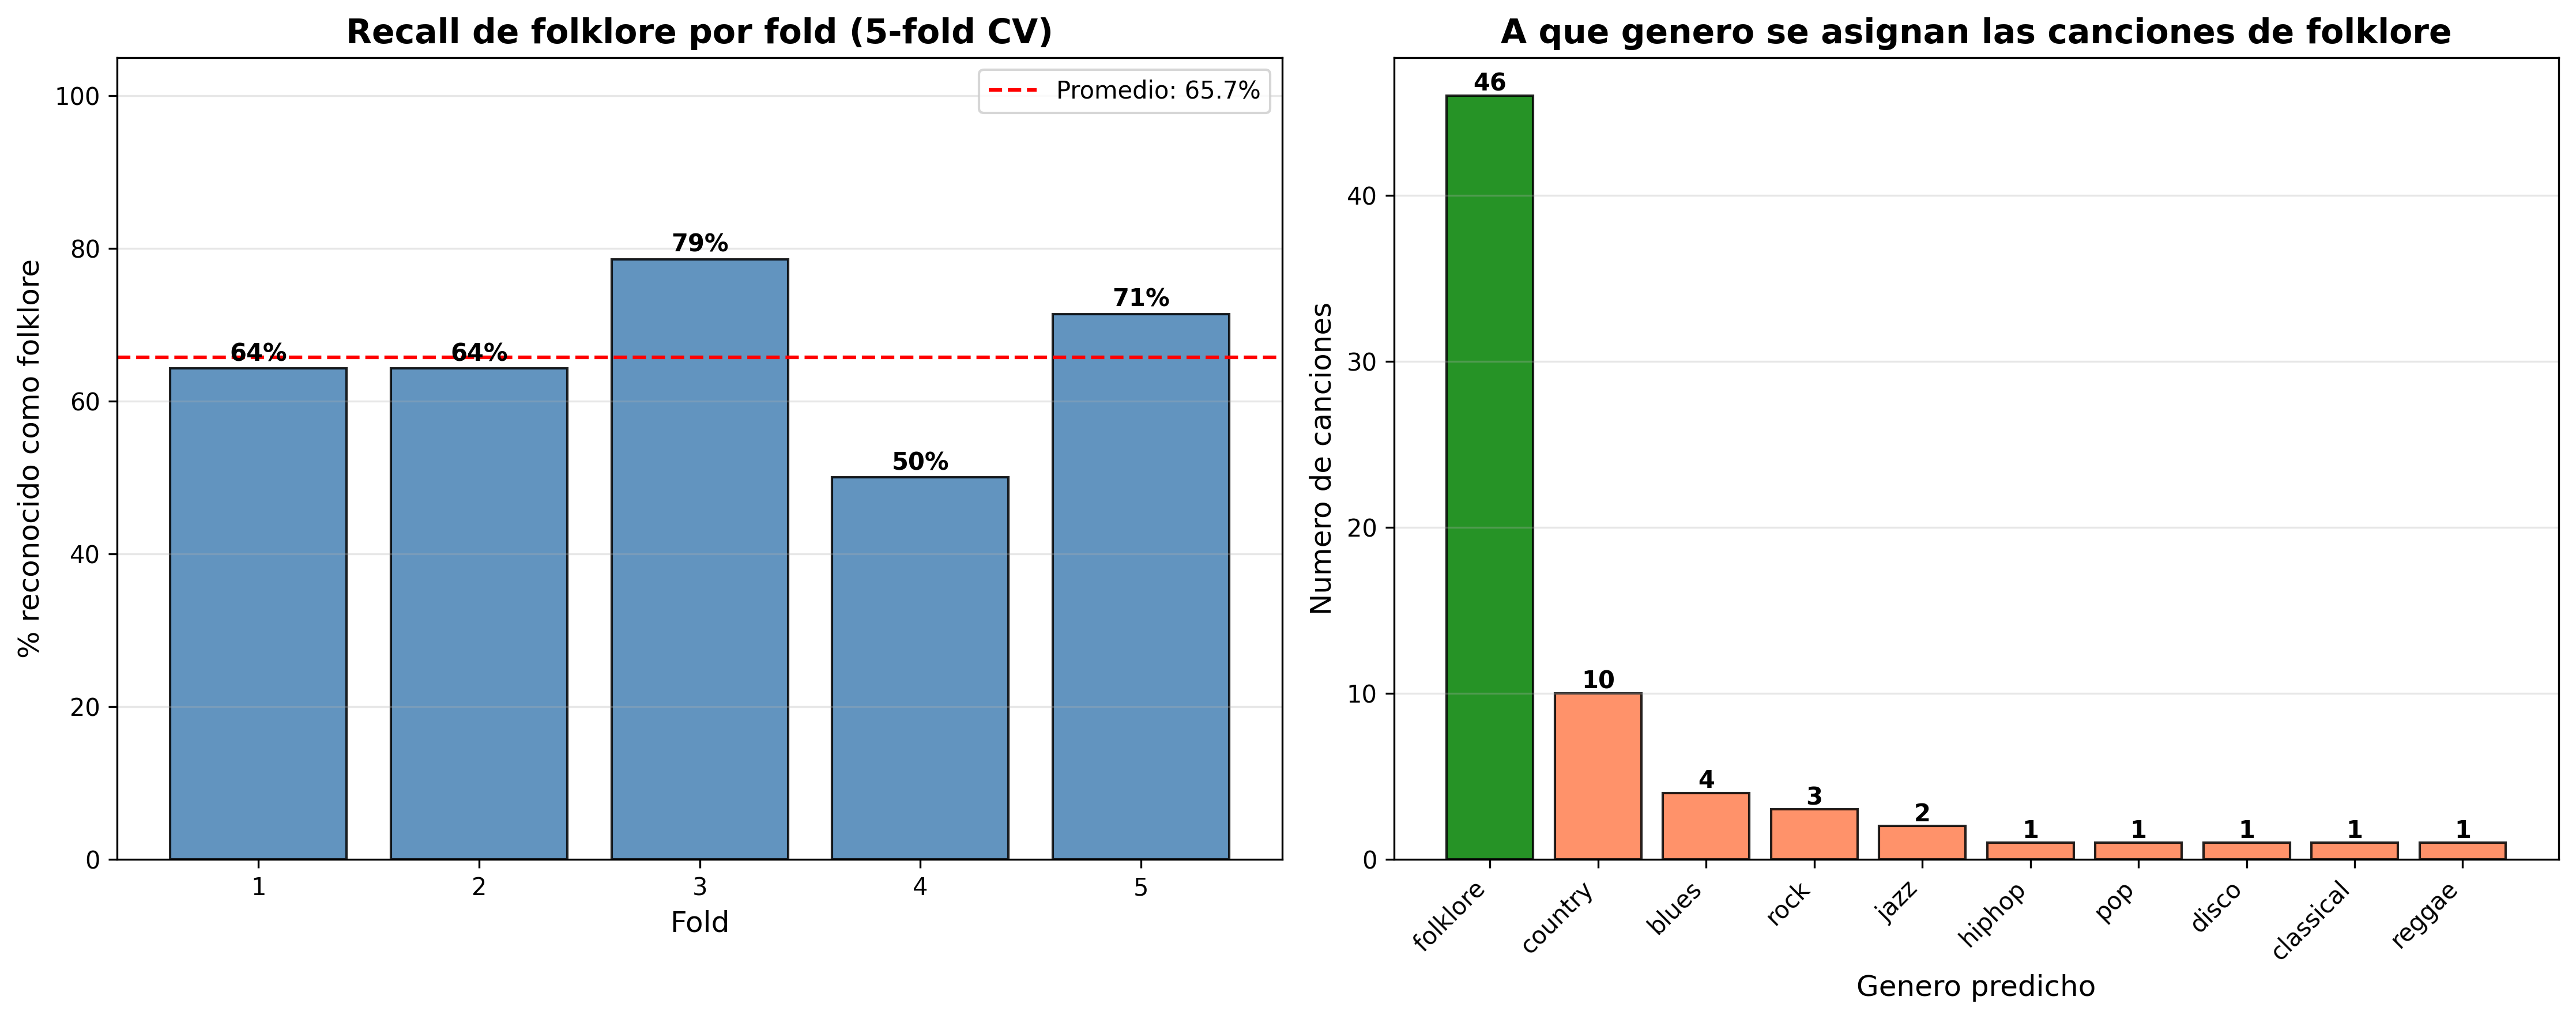
\includegraphics[width=\linewidth]{../results/folklore_crossvalidation.png}
\caption{Validación cruzada del folklore. Izquierda: recall por fold (estable
alrededor del 66\%). Derecha: a qué género se asigna cada canción --- la mayoría
acierta ``folklore'', y los errores caen sobre todo en \emph{country}.}
\end{figure}

\begin{ideabox}{Qué demuestra esto (y cómo conecta con el Experimento A)}
\begin{enumerate}[leftmargin=0.5cm]
  \item \textbf{Las features sí sirven}: con 70 ejemplos el modelo reconoce el
  folklore $\sim$66\% de las veces, muy por encima del azar ($1/11 \approx 9\%$).
  El problema del Experimento A no eran las features, era la \textbf{falta de
  ejemplos}.
  \item \textbf{Confirma la historia acústica}: cuando el modelo \emph{falla},
  el error más frecuente sigue siendo \textbf{country} (10 de 24), seguido de
  blues y rock --- todos géneros de \textbf{guitarra acústica}. Es exactamente lo
  que predecía el Experimento A: el folklore ``suena'' acústicamente parecido al
  country.
  \item \textbf{El número es honesto}: 65.7\% $\pm$ 9.5\% es una métrica
  promediada sobre las 70 canciones, no una corrida con suerte.
\end{enumerate}
\end{ideabox}

\begin{defenbox}{Por qué el folklore es difícil incluso así}
Un 66\% es bueno pero no altísimo, y tiene una explicación de fondo: el folklore
argentino es \textbf{muy heterogéneo} (una chacarera, una zamba y un chamamé
suenan distinto entre sí). Lo estamos forzando a ser \emph{una} clase. Separarlo
en subgéneros, o sumar más canciones, subiría el recall. Es la principal línea
de trabajo futuro.
\end{defenbox}

% ================= 6. RED NEURONAL =================
\section{Modelo 2: Red Neuronal (MLP)}

Para cumplir con el requisito de usar \textbf{al menos dos modelos}, se entrena
un Perceptrón Multicapa (MLP) con Keras sobre las \emph{mismas} 45 features. Vive
dentro del script de comparación (\texttt{6\_model\_comparison.py}), entrenado
sobre el dataset ampliado de 11 clases (GTZAN + folklore).

\begin{lstlisting}
model = keras.Sequential([
    layers.Dense(128, activation='relu', input_shape=(45,)),
    layers.Dropout(0.3),
    layers.Dense(64, activation='relu'),
    layers.Dropout(0.3),
    layers.Dense(32, activation='relu'),
    layers.Dense(11, activation='softmax')   # 11 generos (GTZAN + folklore)
])
\end{lstlisting}

\subsection{Anatomía de la red}

\begin{description}[leftmargin=0.5cm,style=nextline]
  \item[Capa de entrada (45)] Un nodo por feature.
  \item[Capas ocultas (128 $\rightarrow$ 64 $\rightarrow$ 32)] Cada
  \texttt{Dense} aprende combinaciones de la capa anterior. \textbf{ReLU}
  (\(\max(0,x)\)) introduce la no linealidad que permite aprender patrones
  complejos.
  \item[Dropout (0.3)] En cada paso de entrenamiento ``apaga'' al azar el 30\%
  de las neuronas. Esto \textbf{evita el sobreajuste}: la red no puede depender
  de una sola neurona y aprende representaciones más robustas.
  \item[Capa de salida (11, softmax)] \textbf{Softmax} convierte las 11 salidas
  en una distribución de probabilidad que suma 1: ``75\% rock, 15\% metal...''.
\end{description}

\subsection{Cómo aprende}

\begin{itemize}[leftmargin=0.7cm]
  \item \textbf{Loss = categorical\_crossentropy}: mide cuán lejos está la
  probabilidad predicha de la respuesta correcta (one-hot). Entrenar = minimizar
  esta pérdida.
  \item \textbf{Optimizer = adam}: ajusta los pesos por descenso de gradiente con
  tasa de aprendizaje adaptativa.
  \item \textbf{50 epochs}: pasa 50 veces por todo el train. \texttt{validation\_split=0.2}
  reserva 20\% para vigilar el sobreajuste durante el entrenamiento.
\end{itemize}

\subsection{Comparación cualitativa}

\begin{center}
\begin{tabular}{p{4cm} p{5cm} p{5cm}}
\toprule
 & \textbf{SVM (RBF)} & \textbf{Red Neuronal (MLP)} \\
\midrule
Datos ideales & Pocos/medianos & Muchos \\
45 features & Muy cómodo & Funciona, puede sobreajustar \\
Interpretabilidad & Media (vectores de soporte) & Baja (caja negra) \\
Ajuste de hiperparámetros & Pocos ($C$, $\gamma$) & Muchos (capas, dropout, lr) \\
Determinismo & Determinista (semilla fija) & Ruidoso (init aleatoria) \\
\bottomrule
\end{tabular}
\end{center}

\subsection{Comparación justa (mismo dataset y mismo split)}

\begin{defenbox}{Cuidado con las comparaciones tramposas}
Una primera medición ``suelta'' de la red daba \textbf{77\% vs 68\% del SVM},
pero esa comparación era \textbf{inválida}: la red se medía solo sobre GTZAN (10
clases, sin folklore) y con un split \textbf{sin estratificar}, mientras que el
SVM usaba un split estratificado sobre datos distintos. Peras con manzanas. Por
eso ambos modelos se entrenan y evalúan en \textbf{un único script} sobre el
mismo split.
\end{defenbox}

El script \texttt{6\_model\_comparison.py} hace la comparación \textbf{correcta}:
entrena \emph{ambos} modelos sobre el \textbf{mismo} dataset ampliado (GTZAN +
folklore, 11 clases), con el \textbf{mismo} split estratificado 80/20 y el mismo
\texttt{StandardScaler}.

\begin{center}
\begin{tabular}{l c c}
\toprule
\textbf{Métrica} & \textbf{SVM} & \textbf{Red Neuronal} \\
\midrule
Accuracy global & \textbf{68.2\,\%} & 65--68\,\% (varía) \\
Folklore --- precision & 75.0\,\% & $\sim$53\,\% \\
Folklore --- recall & 64.3\,\% (9/14) & 64.3\,\% (9/14) \\
Folklore --- f1-score & 69.2\,\% & 58--72\,\% (varía) \\
\bottomrule
\end{tabular}
\end{center}

\begin{figure}[h]
\centering
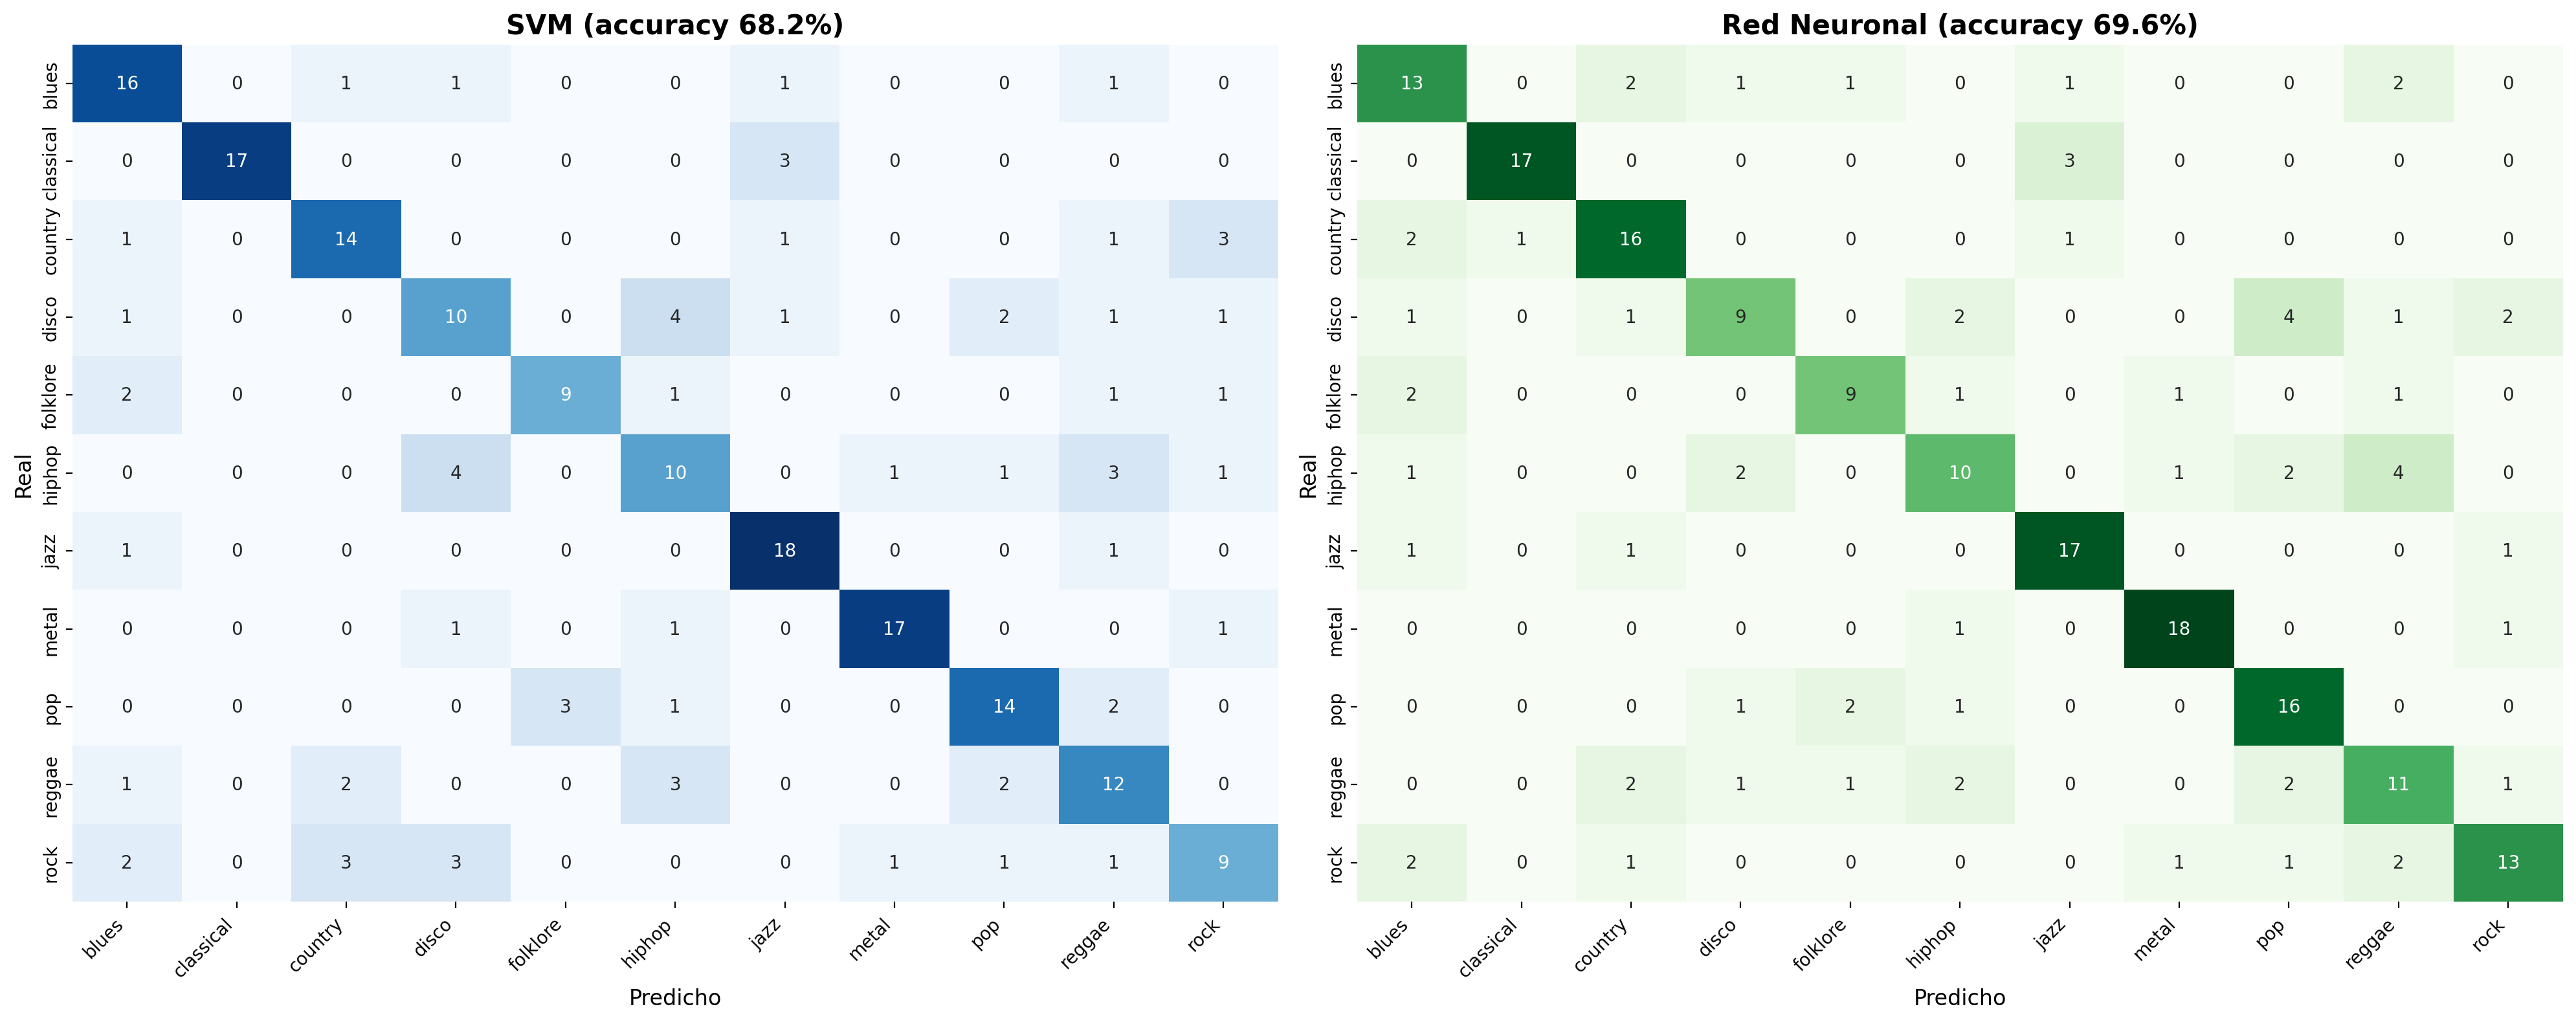
\includegraphics[width=\linewidth]{../results/model_comparison.png}
\caption{Matrices de confusión de ambos modelos sobre el mismo conjunto de test
de 11 clases. Rendimiento muy parecido; el folklore se reconoce de forma similar
en los dos.}
\end{figure}

\begin{ideabox}{Conclusión de la comparación}
Enfrentados de forma justa, \textbf{SVM y red neuronal quedan parejos}
($\sim$66--68\%): la red \textbf{no} es mejor. Es más, el SVM gana levemente y de
forma \emph{estable}, mientras que la red varía entre corridas por su
inicialización aleatoria. La razón de fondo: con un dataset \textbf{chico} (1000
canciones) y features ya ``destiladas'' por \texttt{librosa}, un modelo más
complejo no tiene de dónde sacar ventaja. \textbf{Una buena representación de los
datos (las features) suele importar más que la complejidad del modelo.}
\end{ideabox}

% ================= 7. CNN =================
\section{Modelo 3 (descartado): CNN sobre espectrogramas}

A diferencia de los anteriores, la CNN \textbf{no usa las 45 features}: trabaja
directamente sobre el \textbf{mel-espectrograma} (una imagen
frecuencia $\times$ tiempo de $128 \times 130$). La idea es tratar la
clasificación de audio como \textbf{clasificación de imágenes}.

\begin{itemize}[leftmargin=0.7cm]
  \item Las capas \texttt{Conv2D} aprenden \textbf{sus propios filtros}
  (texturas del espectrograma) en lugar de usar features diseñadas a mano.
  \item \texttt{MaxPooling} reduce la resolución; \texttt{BatchNormalization} y
  \texttt{Dropout} estabilizan y regularizan.
  \item Conserva la \textbf{estructura temporal} que el promedio mean/std
  destruía.
\end{itemize}

\begin{defenbox}{Por qué se descartó (en principio)}
La CNN necesita \textbf{muchos más datos} y cómputo para superar al SVM; con
GTZAN (y solo 100 clips/género) tiende a sobreajustar y no aporta una mejora
clara que justifique la complejidad. Queda documentada como \textbf{línea de
trabajo futuro}, no como resultado principal.
\end{defenbox}

% ================= 8. PREGUNTAS DEFENSA =================
\section{Preguntas probables en la defensa (y cómo responderlas)}

\begin{description}[leftmargin=0.4cm,style=nextline]
  \item[¿Qué hace exactamente \texttt{librosa.load}?] Muestrea el audio a 22050
  Hz y devuelve un arreglo de amplitudes \texttt{y} y el sample rate \texttt{sr}.
  Tomamos 30 s para que todas las canciones sean comparables.

  \item[¿Qué es un MFCC en una frase?] Un conjunto de coeficientes que describen
  la \textbf{forma de la envolvente espectral} en escala perceptual (Mel), es
  decir, el \textbf{timbre} del sonido.

  \item[¿Por qué promedian las features en el tiempo?] Porque el SVM necesita un
  vector de tamaño fijo. Resumimos cada feature temporal con su media y
  desviación estándar, asumiendo el costo de perder la estructura temporal.

  \item[¿Por qué folklore $\rightarrow$ country?] Comparten timbre de guitarra
  acústica (MFCC), armonía simple (chroma) y tempo medio. El modelo compara
  números, no cultura.

  \item[¿Por qué normalizan?] Para que features con escalas grandes (tempo,
  rolloff) no dominen sobre las chicas (ZCR). El scaler se ajusta solo con el
  train para evitar data leakage.

  \item[¿Por qué SVM y no solo red neuronal?] Con un dataset chico y features ya
  informativas, el SVM generaliza muy bien con pocos hiperparámetros. La red
  neuronal se incluye para comparar y necesita más datos.

  \item[¿Es robusto el Experimento B?] El primer script no (test de 1 canción).
  Por eso hicimos la versión correcta (script \texttt{5}) con \textbf{cross-validation
  5-fold} sobre las 70 canciones: recall de folklore \textbf{65.7\% $\pm$ 9.5\%},
  una métrica estable y promediada, no una corrida con suerte.

  \item[¿Qué mejorarían?] Más folklore (50--100), separarlo en subgéneros
  (chacarera, zamba, chamamé), cross-validation, y explorar features temporales
  o una CNN con más datos.
\end{description}

\vspace{0.6cm}
\begin{center}
\rule{0.5\textwidth}{0.4pt}\\[0.3cm]
{\small\itshape Fin de la guía de estudio. ¡Éxitos en la defensa!}
\end{center}

\end{document}
